\documentclass[12pt, oneside]{report}

\usepackage[left=2.5cm, top=2.5cm, bottom=2.5cm, right=2.5cm]{geometry}

\usepackage[utf8]{inputenc}
\usepackage[T1]{polski}
\usepackage[polish]{babel}
\usepackage{hyperref}
\usepackage{physics}
\usepackage{graphicx}
\usepackage{amsthm}
\usepackage{enumitem}
\usepackage{mathtools}
\usepackage{amsfonts}
\usepackage{scalefnt}

\newtheorem{theorem}{Twierdzenie}
\newtheorem{lemma}{Lemat}
\newtheorem{definition}{Definicja}
\newcommand\Omicron{O}
\DeclarePairedDelimiter\floor{\lfloor}{\rfloor}
\newcommand{\nexists}{\not\exists}

\begin{document}  
\thispagestyle{empty}
\begin{titlepage}
    \begin{center}

           \Large
    \textbf{Uniwersytet Jagielloński w Krakowie}\vspace{0.2cm}\\ Wydział Matematyki i Informatyki
               \vspace*{1cm}
               
         \vspace{3cm}
         \Large
          \textbf{Pola Kyzioł}\\\vspace{0.5cm}
         \normalsize Nr albumu: 1092406\\
             \vspace{2cm}
        \Huge
        \textbf{Algorytmy dynamiczne po dekompozycji drzewowej dla problemów grafowych o spójnych rozwiązaniach.}
      
        \vspace{1.5cm}
        \normalsize
        Praca magisterska\\
        na kierunku Informatyka Analityczna\\ \vspace{0.15cm}
        
        \vfill
        \vspace{2cm}
       \begin{minipage}{1\textwidth}
\begin{flushright}
Praca wykonana pod kierunkiem\\
dr. hab. Tomasza Krawczyka\\
Instytut Informatyki Analitycznej 
\end{flushright}
\end{minipage}
        
        \vspace{2cm}
        \begin{center}
      Kraków 2019
        \end{center}
    \end{center}
\end{titlepage}

\newpage 
 \thispagestyle{empty}
\vspace{2.5cm}
\begin{flushleft}
\large \textbf{Oświadczenie autora pracy}\vspace{0.6cm}\\
\end{flushleft}

\noindent Świadom odpowiedzialności prawnej oświadczam, że niniejsza praca dyplomowa została napisana przeze mnie samodzielnie i nie zawiera treści uzyskanych w sposób niezgodny z obowiązującymi przepisami.\\

\noindent Oświadczam również, że przedstawiona praca nie była wcześniej przedmiotem procedur związanych z uzyskaniem tytułu zawodowego w wyższej uczelni.
\vspace{2cm}
\begin{center}
\begin{tabular}{lr}
................................~~~~~~~~~~~~~~~~~~~~~~~~~~~~~~~~~~~~~~&
.......................................... \\
{~~~~Kraków, dnia} & {Podpis autora pracy~~~~}
\end{tabular}
\end{center}
\vspace{5cm}
\begin{flushleft}
\large \textbf{Oświadczenie kierującego pracą}
\end{flushleft}

\noindent Potwierdzam, że niniejsza praca została przygotowana pod moim kierunkiem i~kwalifikuje się do przedstawienia jej w postępowaniu o nadanie tytułu zawodowego.
\vspace{2cm}
\begin{center}
\begin{tabular}{lr}
................................~~~~~~~~~~~~~~~~~~~~~~~~~~~~~~~~~~~~~~&
............................................ \\
{~~~~Kraków, dnia} & {Podpis kierującego pracą~~}
\end{tabular}
\end{center}
\vfill

\newpage
\tableofcontents

\newpage
  	\chapter{Wprowadzenie}
	\emph{Problem Cyklu Hamiltona} oraz \emph{problem Drzewa Steinera} są jednymi z najstarszych i najczęściej badanych problemów należących do klasy problemów $\mathcal{NP}$-zupełnych. Niech $G=(V, E)$ będzie grafem prostym, nieskierowanym. \emph{Cyklem Hamiltona} w grafie $G$ nazywamy cykl długości $\abs{V(G)}$, który przechodzi przez każdy wierzchołek dokładnie jeden raz. Dla zbioru wierzchołków $K \subset V(G)$, \emph{drzewem Steinera} dla zbioru $K$ nazywamy drzewo zawarte w $G$, łączące wszystkie wierzchołki z $K$. Wierzchołki ze zbioru $K$ nazywamy \emph{terminalami}.  
	W niniejszej pracy rozważamy warianty decyzyjne tych problemów. Ich definicje zostały przedstawione poniżej. 
\newline\newline
\textsc{Problem Cyklu Hamiltona}
\newline
\textsc{\scalefont{0.75} Wejście:} Graf $G$.
\newline
\textsc{\scalefont{0.75} Wyjście:} \textsc{tak}, jeżeli w grafie $G$ istnieje cykl Hamiltona.
\newline\newline
\textsc{Problem Drzewa Steinera}
\newline
\textsc{\scalefont{0.75} Wejście:} Graf $G(V,E)$, zbiór wierzchołków terminalnych $K \subset V(G)$, liczba naturalna $\ell$.
\newline
\textsc{\scalefont{0.75} Wyjście:} \textsc{tak}, jeżeli w grafie $G$ istnieje drzewo Steinera dla zbioru $K$ o nie więcej niż $\ell$ krawędziach.
\newline\newline
Dla powyższych problemów istnieją algorytmy dynamiczne po dekompozycji drzewowej, które świadczą, że powyższe problemy należą do klasy problemów FPT, gdzie parametrem jest szerokość drzewowa grafu $G$ danego na wejściu. Klasyczne algorytmy dla tych problemów działają w czasie $k^{\Omicron(k)} \cdot n^{\Omicron{(1)}}$, gdzie $k$ jest \emph{szerokością drzewową grafu $G$}, a $n$ liczbą wierzchołków grafu $G$. Definicje dekompozycji drzewowej oraz szerokości drzewowej są przedstawione w rozdziale~\ref{definitions}. W książce \emph{Parametrized Algorithms} \cite{parametrized_algorithms} autorzy za pracą \cite{solving_connectivity_problems} opisują algorytmy probabilistyczne dla powyższych problemów, które działają w czasie $2^{\Omicron(k)} \cdot n^{\Omicron{(1)}}$. Algorytmy te bazują na technice \emph{Cut \& Count}, która redukuje problem decyzyjny do problemu zliczania rozwiązań modulo $2$. Technika ta jest opisana w rozdziale~\ref{cut_n_count}.

Celem niniejszej pracy jest opis, analiza, implementacja oraz porównanie wydajności klasycznych algorytmów dynamicznych po dekompozycji drzewowej oraz algorytmów probabilistycznych wykorzystujących technikę Cut \& Count dla problemów Cyklu Hamiltona oraz Drzewa Steinera. 

Wszystkie powyższe algorytmy zostały zaimplementowane w języku programowania C++ oraz przetestowane. Testy wydajnościowe zostały przeprowadzone na wygenerowanych instancjach dekompozycji drzewowych, ich wyniki są zobrazowane na wykresach przedstawionych w rozdziale \ref{summary}. Implementacja algorytmów jest udostępniona w repozytorium na githubie~\cite{github}. Wszystkie instancje wejściowe dekompozycji drzewowych można wyeksportować do plików .dot, a następnie wygenerować z nich wizualizacje drzew. Więcej informacji na temat biblioteki znajduje się w pliku README.txt dostępnym w repozytorium.  

\newpage
  	\chapter{Podstawowe definicje}
  	\label{definitions}
	
\begin{definition}
\em \emph{Dekompozycją drzewową grafu} $G$ nazywamy parę $\mathcal{T} = (T, \{X_t : t \in V(T)\})$, gdzie $T$ jest drzewem, a $\{X_t : t \in V(T)\}$ rodziną zbiorów wierzchołków grafu $G$ spełniającą następujące warunki:
\begin{enumerate}[label=(\roman*)]
	\item{Dla każdej krawędzi $\{u, v\} \in E(G)$ istnieje węzeł $t \in V(T)$, taki że $u \in X_t$ i $v \in X_t$.}
	\item{Dla każdego wierzchołka $v \in V(G)$ zbiór $\{t \in V(T): v \in X_t \}$ jest poddrzewem drzewa $T$.}
\end{enumerate}
\end{definition}

Od tej pory wierzchołki grafu $G$ będą nazywane po prostu \emph{wierzchołkami}, natomiast wierzchołki $t$ drzewa $T$ oraz zbiory $X_t$ będą nazywane \emph{węzłami} $\mathcal{T}$.

\begin{definition}
\em \emph{Szerokość drzewowa dekompozycji drzewowej $\mathcal{T}=(T, \{X_t : t \in V(T)\})$}, oznaczana przez $sd_\mathcal{T}$, to rozmiar najliczniejszego węzła $\mathcal{T}$ pomniejszony o $1$, to jest: $$sd_\mathcal{T} = max_{t \in V(T)} \abs{X_t} - 1.$$ 
\end{definition}

\begin{definition}
\em \emph{Szerokość drzewowa grafu $G$}, standardowo oznaczana przez $sd_G$ lub $k$, jest minimalną szerokością drzewową wziętą po wszystkich możliwych dekompozycjach drzewowych $G$: $$sd_G = min \{sd_\mathcal{T}: \mathcal{T} \text{ jest dekompozycją drzewową }G\}.$$
\end{definition}

Przy konstruowaniu algorytmów dynamicznych działających po dekompozycji drzewowej grafu łatwiej jest posługiwać się tzw. \emph{ładną dekompozycją drzewową}.

\begin{definition}
\em Dekompozycja drzewowa $\mathcal{T} = (T, \{X_t\}_{t \in V(T)})$ jest \emph{ładna}, jeżeli $\mathcal{T}$ spełnia następujące własności:
\begin{enumerate}[label=(\roman*)]
	\item{$T$ jest drzewem ukorzenionym z korzeniem w węźle $r$.}
	\item{Każdy węzeł $t \in T$ ma jeden z następujących pięciu typów:}
	\begin{enumerate}[label=\arabic*)]
		\item{$t$ jest \texttt{LIŚCIEM}, jeżeli $t$ jest liściem w $T$ i $X_t = \emptyset$.}
		\item{$t$ jest \texttt{WĘZŁEM WPROWADZAJĄCYM WIERZCHOŁEK} $v$, jeżeli $t$ ma jedno dziecko $t'$ oraz zachodzi zależność $X_t = X_{t'} \cup \{v\}$ oraz $v \notin X_{t'}$. Każdy wierzchołek $v \in V(G)$ ma co najmniej jeden węzeł wprowadzający wierzchołek $v$.}
		\item{$t$ jest \texttt{WĘZŁEM ZAPOMINAJĄCYM WIERZCHOŁEK} $v$, jeżeli $t$ ma jedno dziecko $t'$ oraz zachodzi zależność $X_t = X_{t'} \setminus \{v\}$ oraz $v \in X_t$. Jego szczególnym reprezentantem jest korzeń. Dla każdego wierzchołka $v \in V(G)$ istnieje dokładnie jeden węzeł zapominający.}
		\item{$t$ jest \texttt{WĘZŁEM SCALAJĄCYM}, jeżeli $t$ posiada dwoje dzieci oraz zachodzi zależność $X_t = X_{t'} = X_{t''}$.}
		\item{$t$ jest \texttt{WĘZŁEM WPROWADZAJĄCYM KRAWĘDŹ} $uv$, jeżeli $t$ ma jedno dziecko $t'$ oraz zachodzi zależność $X_t = X_{t'}$. Dla każdej krawędzi $uv$ grafu $G$ wymagamy, aby krawędź ta była wprowadzona dokładnie jeden raz, tuż przed pierwszym ,,zapomnieniem'' jednego z wierzchołków $u$ lub $v$.}
\end{enumerate}
\end{enumerate}
\end{definition}

\begin{definition}
\em Dla węzła $t$ definiujemy graf $G_t = (V_t, E_t)$, gdzie: 
\begin{itemize}[noitemsep,topsep=5pt,parsep=0pt,partopsep=0pt]
\item[$V_t$]{jest zbiorem wierzchołków wprowadzonych w poddrzewie ukorzenionym w $t$.}
\item[$E_t$]{jest zbiorem krawędzi wprowadzonych w poddrzewie ukorzenionym w $t$.} 
\end{itemize}
\end{definition}

\begin{figure}
\centering
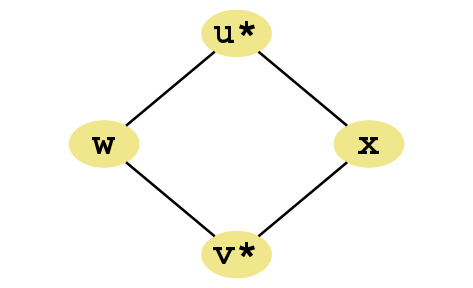
\includegraphics[width=5cm]{square_steiner_tree_standard_graph.png}
\caption{Przykładowy graf $G$.}
\label{kwadrat}
\end{figure}

\begin{figure}
\centering
\makebox[\textwidth]{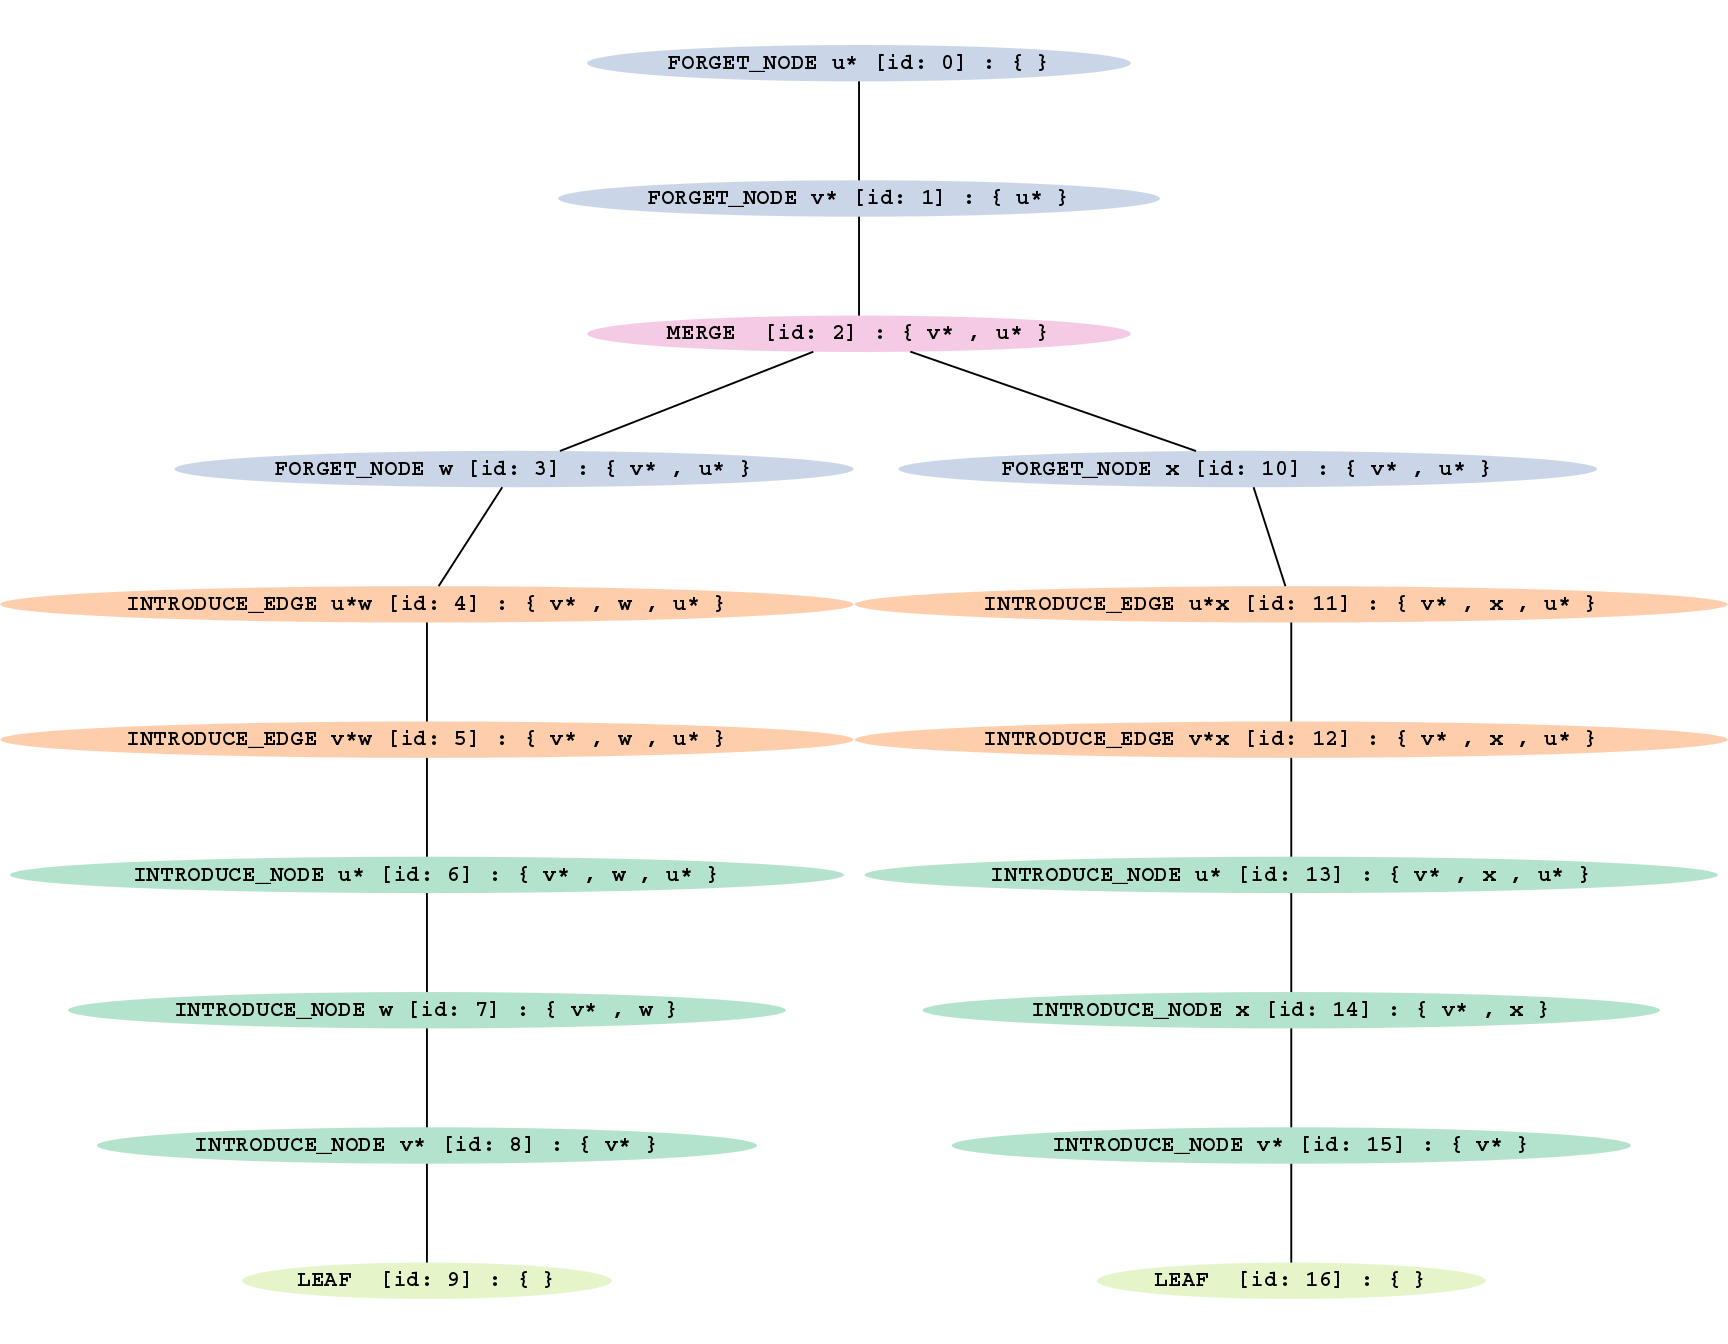
\includegraphics[width=18cm, height=14cm]{square_steiner_tree_standard.png}}
\caption{Ładna dekompozycja drzewowa grafu $G$ z rys. \ref{kwadrat}. Wierzchołki terminalne są oznakowane *.}
\label{dekompozycja_kwadratu}
\end{figure}

Problem obliczania dekompozycji drzewowej należy do klasy problemów FPT, gdzie parametrem jest szerokość drzewowa grafu wejściowego (Bodlaender \cite{bodlaender}). Kloks~\cite{kloks} pokazał, że dla każdego grafu o szerokości drzewowej $k$ istnieje ładna dekompozycja drzewowa o szerokości drzewowej $k$, którą można skonstruować w czasie liniowym od liczby wierzchołków grafu $G$.
\newline\newline
\noindent W naszej pracy rozważać będziemy następujące problemy.

\begin{definition}
\em \emph{Problem Drzewa Steinera.} Na wejściu mamy dany graf $G$ wraz z jego ładną dekompozycją drzewową $\mathcal{T} = (T, \{X_t\}_{t \in V(T)})$, zbiór terminali $K \subseteq V(G)$ oraz liczbę naturalną $\ell$. Pytamy, czy istnieje drzewo Steinera dla zbioru terminali $K$ składające się z co najwyżej $\ell$ krawędzi.
\end{definition}

\begin{definition}
\em \emph{Problem Cyklu Hamiltona.} Na wejściu mamy dany graf $G$ wraz z jego ładną dekompozycją drzewową $\mathcal{T} = (T, \{X_t\}_{t \in V(T)})$. Pytamy, czy istnieje cykl Hamiltona w grafie $G$.
\end{definition}

\newpage
  	\chapter{Klasyczne algorytmy dynamiczne}
    	\section{Drzewo Steinera}
    	
W tym rozdziale zostanie przedstawiony klasyczny algorytm dynamiczny po dekompozycji drzewowej dla problemu Drzewa Steinera.

W celu uproszczenia algorytmu, przyjmujemy, że każdy węzeł drzewa $T$ zawiera przynajmniej jeden terminal. W tym celu wybieramy dowolny wierzchołek $v_0 \in K$ i dodajemy go do każdego węzła dekompozycji $\mathcal{T}$. Własności ładnej dekompozycji drzewowej są zachowane z modyfikacją, że szerokość drzewowa $\mathcal{T}$ wzrasta o $1$ oraz węzły będące liśćmi i korzeniem zawierają wierzchołek $v_0$.

\begin{figure}
\centering
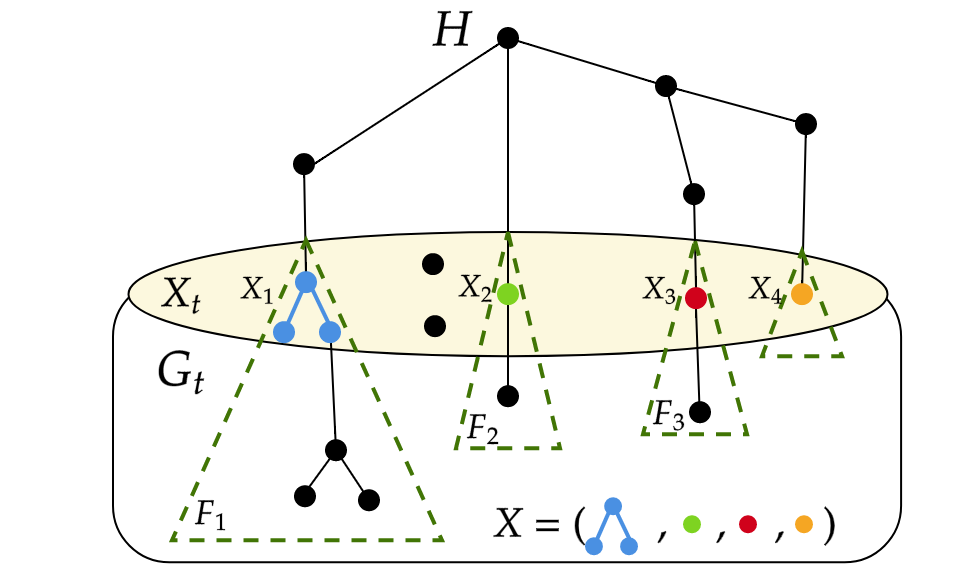
\includegraphics[width=16cm]{steiner_tree.png}
\caption{Przykładowy ślad drzewa Steinera w węźle $t$.}
\label{steiner_tree}
\end{figure}

Zastanówmy się, jaki ślad na grafie $G_t = (V_t, E_t)$ zostawia potencjalne drzewo Steinera dla zbioru terminali $K$. Załóżmy, że $H$ jest takim drzewem Steinera. Niech $\mathcal{F} = (V_t \cap V(H), E_t \cap E(H))$ będzie podgrafem $G_t$ składającym się z wierzchołków i krawędzi należących do $H$ (patrz rys. \ref{steiner_tree}). Zauważmy, że $\mathcal{F}$ jest lasem. Niech $F_1, F_2, \ldots, F_s$ będą składowymi spójnymi lasu $\mathcal{F}$. Niech $X$ oraz $X_1, X_2, \ldots, X_s$ będą zawężeniami zbiorów $V(F)$ i $V(F_1), \ldots, V(F_s)$ do zbioru $X_t$. Zauważmy, że zbiory $X_1, X_2, \ldots, X_s$ są niepuste, $X_1, X_2, \ldots, X_s$ tworzy podział $X$ oraz $v_0 \in X$ (a w zasadzie $K \cap X_t \subseteq X$).

Klasyczny algorytm dynamiczny dla problemu drzewa Steinera dla każdego węzła $t$, każdego zbioru $X \subseteq X_t$ takiego że $v_0 \in X$ oraz każdego podziału $\mathcal{P}$ zbioru $X$ oblicza wartość $c(t, X, \mathcal{P})$ równą najmniejszej liczbie krawędzi w lesie $\mathcal{F}$ grafu $G_t$, którego spójne składowe w zawężeniu do zbioru $X_t$ pokrywają się ze zbiorami $X_1, X_2, \ldots, X_s$. Algorytm przypisuje $c(t, X, \mathcal{P}) = \infty$, jeżeli drzewo o powyższych własnościach nie istnieje.

Dla kolejnych typów węzłów $t$ dekompozycji $\mathcal{T}$ algorytm działa zgodnie z poniżej zdefiniowanymi formułami rekurencyjnymi. Wynik końcowy odpowiada wartości $c(r, \{v_0\}, \{\{v_0\}\})$. Dla parametrów niezdefiniowanych poniżej, $c(t, X, \mathcal{P})$ przyjmuje wartość $\infty$.
\newline\newline
$t$ jest \texttt{LIŚCIEM}. W tym przypadku należy ustawić:
$$c(t, \{v_0\}, \{\{v_0\}\}) = 0.$$
\newline
$t$ jest \texttt{WĘZŁEM WPROWADZAJĄCYM WIERZCHOŁEK} $v$. Przypomnijmy, że $v$ jest wierzchołkiem izolowanym w $G_t$. Wobec tego, jeżeli $v$ jest w zbiorze co najmniej dwuelementowym podziału $\mathcal{P}$, wtedy $c(t, X, \mathcal{P}) = \infty$. Zauważmy, że jeśli $v$ jest terminalem, $v$ musi należeć do $X$. W zależności od tego, czy $v$ należy do $X$, wartość $c(t, X , \mathcal{P})$ obliczamy zgodnie z regułą:
\[
c(t, X, \mathcal{P}) =  
\left \{
  \begin{tabular}{ccc}
  $c(t', X \setminus \{v\}, \mathcal{P} \setminus \{\{v\}\})$ & jeśli $v \in X$,\\
  $c(t', X, \mathcal{P})$ & jeśli $v \notin X \wedge v \notin K$.
  \end{tabular}
\right. 
\]
\newline
t jest \texttt{WĘZŁEM WPROWADZAJĄCYM KRAWĘDŹ} $uv$. Rozważmy trzy przypadki:

\begin{enumerate}
\item \label{notinx} $u \notin X$ lub $v \notin X$.
\item \label{notinthesamecomponent} $u \in X$, $v \in X$ oraz $u$ i $v$ są w różnych komponentach $\mathcal{P}$ ($u \in X_i$, $v \in X_j$, $i \neq j$).
\item \label{edgepossible} $u \in X$, $v \in X$ oraz $u$ i $v$ są w tych samych komponentach $\mathcal{P}$ ($u,v \in X_i$).
\end{enumerate} 

\noindent W przypadkach \ref{notinx} oraz \ref{notinthesamecomponent} krawędź $uv$ nie może należeć do lasu $\mathcal{F}$, zatem musimy ustawić: 
$$c(t, X, \mathcal{P}) = c(t', X, \mathcal{P}).$$
Natomiast w przypadku \ref{edgepossible} mamy dwie możliwości - albo krawędź $uv$ jest w zbiorze $\mathcal{F}$, albo nie. Jeśli nie dodajemy krawędzi do $\mathcal{F}$, przepisujemy wynik z węzła $t'$, to jest $c(t, X, \mathcal{P}) = c(t', X, \mathcal{P})$. W przeciwnym przypadku krawędź $uv$ musiała połączyć dwa rozłączne bloki podziału $\mathcal{P}'$ węzła $t'$. Ponieważ optymalizujemy po rozmiarze śladu, iterujemy się po wszystkich takich partycjach $\mathcal{P}'$ węzła $t'$, w których $u$ i $v$ nie należą do tego samego komponentu, ale po połączeniu komponentów je zawierających otrzymujemy podział $\mathcal{P}$. Wobec tego $c(t, X, \mathcal{P})$ obliczamy zgodnie z regułą:
$$c(t, X, \mathcal{P}) = \min \big\{ \min\limits_{\mathcal{P}'} c(t', X, \mathcal{P}') + 1, \quad c(t', X, \mathcal{P}) \big\},$$ gdzie $\mathcal{P'}$ oznacza podziały opisane powyżej.
\newline\newline
$t$ jest \texttt{WĘZŁEM ZAPOMINAJĄCYM WIERZCHOŁEK} $v$. Zauważmy, że las $\mathcal{F}$ może być rozłączny z wierzchołkiem $v$, i wtedy: $c(t, X, \mathcal{P}) = c(t', X, \mathcal{P})$.
W przeciwnym przypadku spójna składowa $\mathcal{F}$ zawierająca wierzchołek $v$ musi zawierać jeszcze jeden wierzchołek należący do $X_t$. Prowadzi to do wzoru:
$$c(t, X, \mathcal{P}) = \min \big\{ \min\limits_{\mathcal{P}'} c(t', X \cup \{v\}, \mathcal{P}'), \quad c(t', X, \mathcal{P}) \big\},$$ gdzie $\mathcal{P'}$ przebiega wszystkie podziały $X \cup \{v\}$, w których wierzchołek $v$ jest w zbiorze co najmniej dwuelementowym, a podział $\mathcal{P}'$ po usunięciu $v$ jest równy $\mathcal{P}$.
\newline\newline
\begin{figure}
\centering
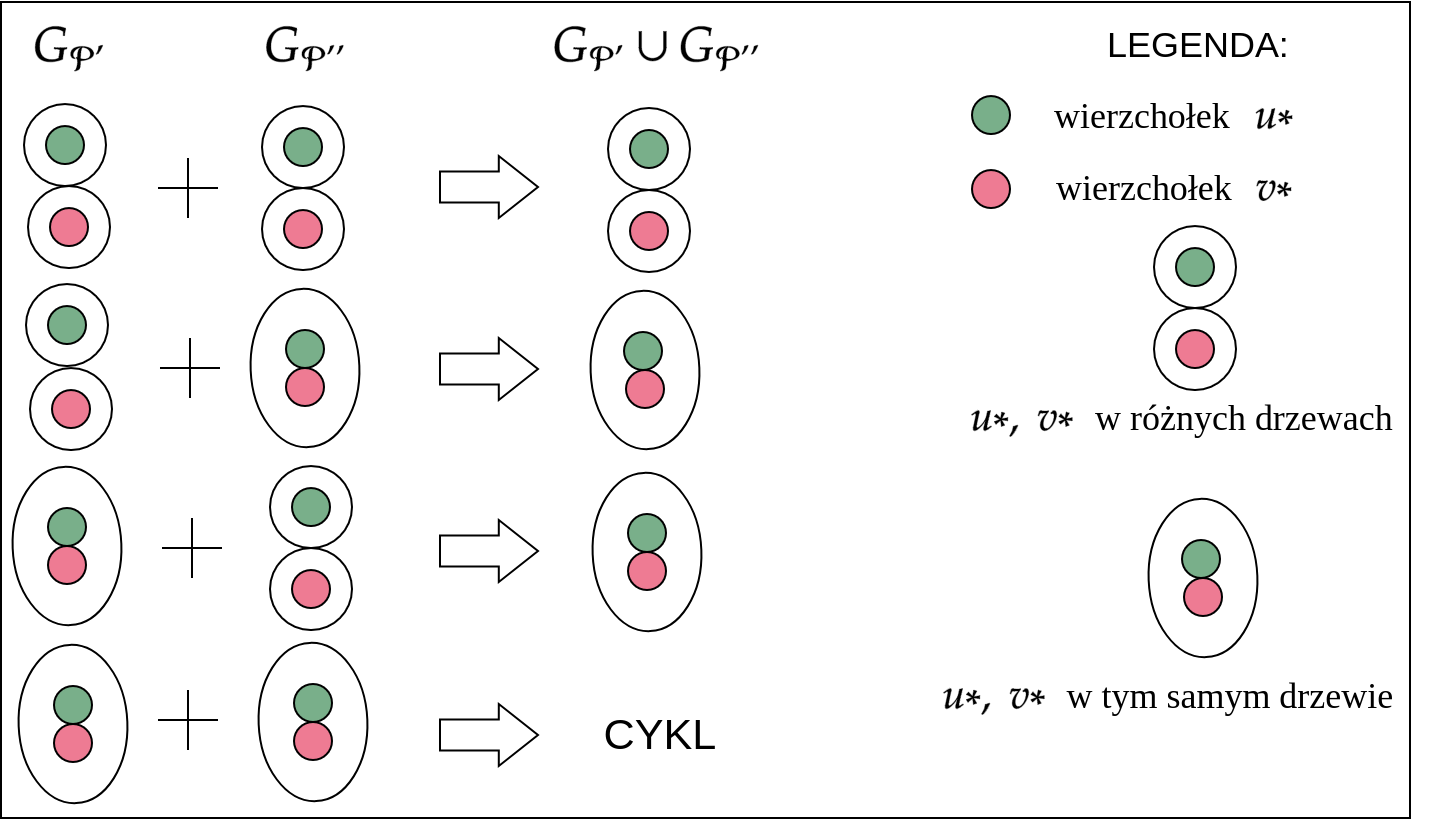
\includegraphics[width=16cm]{find_n_union.png}
\caption{Rezultaty otrzymane w wyniku połączenia lasów $G_{\mathcal{P}'}$, $G_{\mathcal{P}''}$ w węźle scalającym z rys. \ref{dekompozycja_kwadratu}.}
\label{find_n_union}
\end{figure}

\noindent $t$ jest \texttt{WĘZŁEM SCALAJĄCYM}. Zauważmy, że $E_{t'} \cap E_{t''} = \emptyset$. Poszukiwany las jest sumą dwóch lasów: $\mathcal{F}'$ w grafie $G_{t'}$ oraz $\mathcal{F}''$ w grafie $G_{t''}$. Podziały $\mathcal{P}'$ i $\mathcal{P}''$ odpowiadające lasom $\mathcal{F}'$ i $\mathcal{F}''$ spełniają następującą własność. Niech $G_{\mathcal{P}'}$ i $G_{\mathcal{P}''}$ będą lasami o zbiorach wierzchołków odpowiednio $X_{t'}$ oraz $X_{t''}$, których drzewa korespondują z podziałem $\mathcal{P'}$ i $\mathcal{P''}$. Połączenie lasów $G_{\mathcal{P}'}$ i $G_{\mathcal{P}''}$ jest lasem odpowiadającym podziałowi $\mathcal{P}$.

W implementacji powyższego algorytmu do reprezentowania problemu łączenia lasów $G_{\mathcal{P}'}$, $G_{\mathcal{P}''}$ wykorzystałam strukturę zbiorów rozłącznych z łączeniem według rangi i kompresją ścieżek. Dzięki niej łatwo wykryć cykl oraz zbadać, które wierzchołki są w tych samych, spójnych komponentach $\mathcal{P}$. Rysunek \ref{find_n_union} przedstawia wszystkie możliwe lasy $G_{\mathcal{P}'}$, $G_{\mathcal{P}''}$ dla węzła scalającego z rysunku \ref{dekompozycja_kwadratu} wraz z rezultatami połączenia lasów.
Końcowe rozwiązanie wyliczamy na podstawie poniższego wzoru:
$$c(t, X, \mathcal{P}) = \min \limits_{\mathcal{P}', \mathcal{P}''} c(t', X, \mathcal{P}') + c(t'', X, \mathcal{P}''),$$ gdzie $\mathcal{P}'$ i $\mathcal{P''}$ spełniają wyżej przedstawioną zależność.

Przedstawione zostały formuły rekurencyjne dla wszystkich typów węzłów. Przejdźmy zatem do wyliczenia złożoności czasowej standardowego algorytmu dynamicznego po dekompozycji drzewowej dla problemu drzewa Steinera. Poniżej znajdują się istotne spostrzeżenia:
\begin{enumerate}[label=(\alph*)]
\item Każdy węzeł ma co najwyżej $k+2$ wierzchołki.
\item Wszystkich zbiorów $X \subseteq X_t$ jest $2^{\abs{X_t}}$ a zatem nie więcej niż $2^{k+2}$.
\item Wszystkich podziałów $X$ jest rzędu $\abs{X}^{\abs{X}}$, a zatem nie więcej niż $(k+2)^{k+2}$.
\item Dla każdego węzła mamy $2^{k+2} \cdot (k+2)^{k+2} = k^{\Omicron(k)}$ stanów.
\item Wartości funkcji $c$ dla każdego węzła wyliczamy w czasie $(k^{\Omicron(k)})^2$.
\end{enumerate}
Spostrzeżenia nasze możemy podsumować następującym twierdzeniem. 
\begin{theorem}
Mając dany $n$-wierzchołkowy graf $G$ razem ze zbiorem terminali $K \subseteq V(G)$ oraz dekompozycją drzewową o szerokości drzewowej nie większej niż $k$, rozmiar minimalnego drzewa Steinera można wyliczyć w czasie $k^{\Omicron(k)} \cdot n^{\Omicron{(1)}}$. 
\end{theorem}

    	\section{Cykl Hamiltona}
    	
W tym rozdziale przedstawimy klasyczny algorytm dynamiczny po dekompozycji drzewowej dla problemu cyklu Hamiltona. 

Zakładamy, że mamy daną ładną dekompozycję drzewową $\mathcal{T} = (T, \{X_t\}_{t \in V(T)})$ lekko zmodyfikowanego grafu $G$. Modyfikacja polega na tym, że kopiujemy wierzchołek $v_r$, będący w korzeniu dekompozycji drzewowej grafu $G$ (\texttt{WĘZEŁ ZAPOMINAJĄCY WIERZCHOŁEK} $v_r$) wraz z jego krawędziami, tj. dla każdej krawędzi $uv_r \in E(G)$ dodajemy dwie krawędzie $uv_{r_1}$ i $uv_{r_2}$, gdzie $v_{r_1}$ jest byłym wierzchołkiem $v_r$, a $v_{r_2}$ jego kopią. Wtedy, problem istnienia cyklu Hamiltona w $G$ jest równoważny problemowi istnienia ścieżki Hamiltona o końcach $v_{r_1}$ i $v_{r_2}$.

Zastanówmy się, jaki ślad na grafie $G_t$ zostawia potencjalna ścieżka Hamiltona łącząca wierzchołki $v_{r_1}$ i $v_{r_2}$. Niech $H$ będzie taką ścieżką (patrz rys. \ref{hamiltonian}). Niech $\mathcal{P} = (V_t \cap V(H), E_t \cap E(H))$ będzie zawężeniem $H$ do grafu $G_t$. Zauważmy, że $\mathcal{P}$ jest kolekcją ścieżek $P_1, P_2, \ldots, P_s$ w grafie $G$. $H$ jest spójne, co implikuje, że każda ścieżka $P_1, P_2, \ldots, P_s$ przecina $X_t$. Niech $X_{t_0}$, $X_{t_1}$, $X_{t_2}$ będą podzbiorami wierzchołków ze zbioru $X_t$ o stopniach odpowiednio $0$, $1$, $2$ w grafie $\mathcal{P}$. Niech $\mathcal{M}$ będzie dopasowaniem doskonałym na zbiorze wierzchołków $X_{t_1}$, które łączy wierzchołki $u$ i $v$ jeśli $u$ i $v$ są końcami jakiejś ścieżki z $\mathcal{P}$. Zauważmy, że $\mathcal{P}$, $X_{t_0}$, $X_{t_1}$, $X_{t_2}$, $\mathcal{M}$ spełniają następujące własności:
\begin{enumerate}[label=(\roman*)]
\item \label{i}{Każdy wierzchołek ze zbioru $V_t \setminus X_t$ należy do wnętrza jednej ze ścieżek $\mathcal{P}$.}
\item{$X_{t_0} \cup X_{t_1} \cup X_{t_2} = X_t$.}
\item \label{iii}{$\mathcal{M}$ jest dopasowaniem doskonałym na zbiorze $X_{t_1}$, spełniającym własność, że dla każdego $\{u, v\} \in \mathcal{M}$ istnieje ścieżka w $\mathcal{P}$ o końcach $u$ i $v$.}
\end{enumerate} 

\begin{figure}
\centering
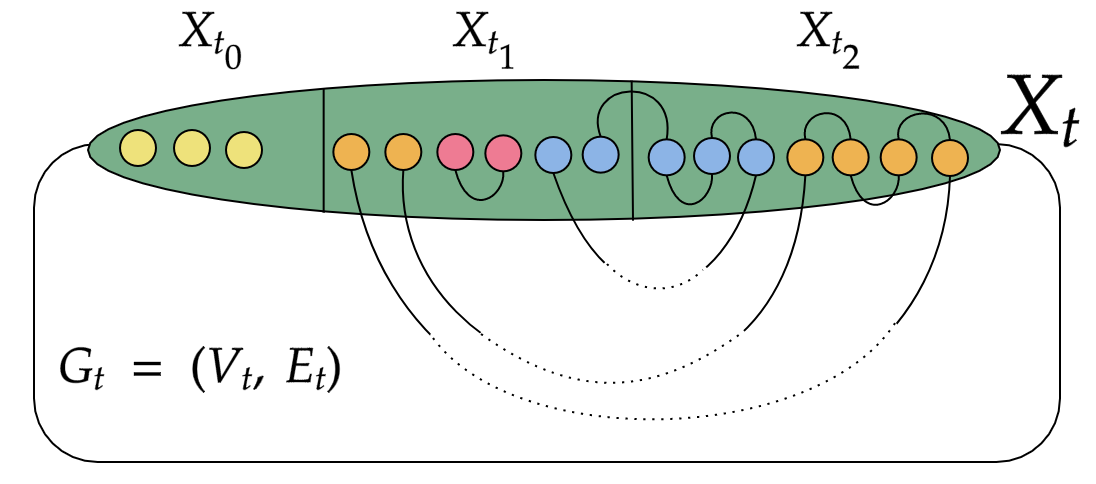
\includegraphics[width=16cm]{hamiltonian.png}
\caption{Przykładowy ślad ścieżki Hamiltona dla węzła $t$.}
\label{hamiltonian}
\end{figure} 

Klasyczny algorytm dynamiczny po dekompozycji drzewowej dla problemu cyklu Hamiltona, dla każdego węzła $t$, dla każdego podziału zbioru $X_t$ na zbiory $X_{t_0}$, $X_{t_1}$, $X_{t_2}$, dla każdego dopasowania $\mathcal{M}$ na zbiorze $X_{t_1}$ sprawdza, czy istnieje pokrycie ścieżkowe $\mathcal{P}$ grafu $G_t$, które spełnia własności \ref{i}-\ref{iii}. Jeśli tak, $c(t, (X_{t_0}, X_{t_1}, X_{t_2}), \mathcal{M})$ przyjmuje wartość \emph{true}, natomiast jeśli takie pokrycie nie istnieje, $c(t, (X_{t_0}, X_{t_1}, X_{t_2}), \mathcal{M})$ przyjmuje wartość \emph{false}. Wynik końcowy odpowiada wartości $c(r, (\emptyset, \{v_{r_1}, v_{r_2}\}, \emptyset), \{\{v_{r_1}, v_{r_2}\}\})$. Poniżej prezentuję formuły rekurencyjne obliczania wartości funkcji $c$ ze względu na typ węzła $t$. Wartość funkcji $c$ dla parametrów niezdefiniowanych poniżej wynosi $false$.
\newline\newline
$t$ jest \texttt{LIŚCIEM}. Dla tego przypadku należy ustawić:
$$c(t, (\emptyset, \emptyset, \emptyset), \emptyset) = true.$$
\newline
$t$ jest \texttt{WĘZŁEM WPROWADZAJĄCYM WIERZCHOŁEK} $v$. Zaobserwujmy, że w momencie dodawania wierzchołka jego stopień wynosi $0$, wobec czego znajduje się on w zbiorze $X_{t_0}$, co daje nam następującą funkcję rekurencyjną:
\[
c(t, (X_{t_0}, X_{t_1}, X_{t_2}), \mathcal{M}) =  
  \begin{tabular}{ccc}
  $c(t', (X_{t_0} \setminus \{v\}, X_{t_1}, X_{t_2}), \mathcal{M})$ & jeśli $v \in X_{t_0}$.\\
  \end{tabular}
\]
\newline
$t$ jest \texttt{WĘZŁEM ZAPOMINAJĄCYM WIERZCHOŁEK} $v$. Przypomnijmy, że wszystkie krawędzie incydentne do zapominanego wierzchołka zostały już wprowadzone. Ślad jest poprawny tylko wtedy, kiedy zapominany wierzchołek jest stopnia $2$, co prowadzi do następującej formuły:

$$c(t, (X_{t_0}, X_{t_1}, X_{t_2}), \mathcal{M}) = c(t', (X_{t_0}, X_{t_1}, X_{t_2} \cup \{v\}), \mathcal{M}).$$
\begin{figure}
\centering
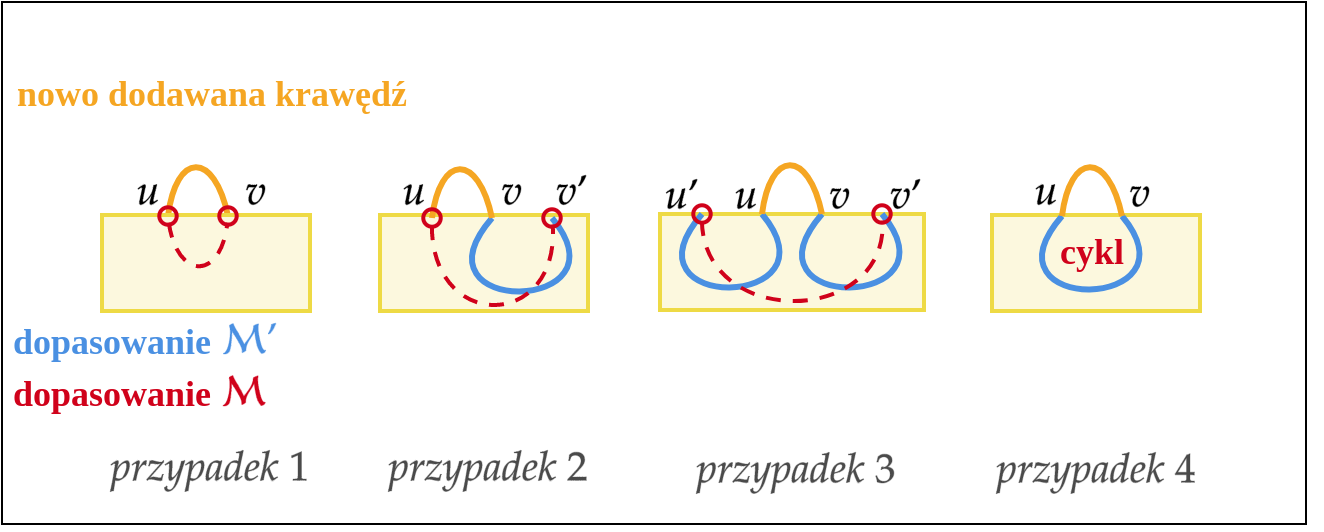
\includegraphics[width=16cm]{introduce_edge.png}
\caption{Dodawanie nowej krawędzi $uv$ do dopasowania $M$.}
\label{introduce_edge}
\end{figure}
$t$ jest \texttt{WĘZŁEM WPROWADZAJĄCYM KRAWĘDŹ} $uv$. Zauważmy, że jeśli krawędź $uv$ zamyka jedną ze ścieżek pokrycia ścieżkowego $\mathcal{P}'$, tworząc cykl, nie może ona należeć do pokrycia ścieżkowego $\mathcal{P}$, i wtedy:
$$c(t, (X_{t_0}, X_{t_1}, X_{t_2}), \mathcal{M}) = c(t', (X_{t_0}, X_{t_1}, X_{t_2}), \mathcal{M}).$$
Taką samą formułę rekurencyjną aplikujemy, kiedy co najmniej jedno z $u$, $v$ należy do $X_{t_0}$.  W pozostałych przypadkach wartości $c(t, (X_{t_0}, X_{t_1}, X_{t_2}), \mathcal{M})$ obliczamy, patrząc zarówno na pokrycia ścieżkowe $\mathcal{P}'$ bez krawędzi $uv$, jak i na pokrycia ścieżkowe z dodaną krawędzią $uv$. Zauważmy, że krawędź $uv$ rozszerza pokrycie ścieżkowe $\mathcal{P}'$ węzła $t'$ w jeden z poniżej przedstawionych sposobów (zobrazowanych na rys. \ref{introduce_edge}):
\begin{enumerate}
\item \label{i_uv}Poprzez połączenie dwóch wierzchołków izolowanych $u$ i $v$, gdzie $u \in X_{t'_0}$ oraz $v \in X_{t'_0}$.
\item Poprzez rozszerzenie istniejącej ścieżki, gdzie $u \in X_{t'_0}$ oraz $v \in X_{t'_1}$ (lub odwrotnie).
\item \label{iii_uv}Poprzez połączenie dwóch istniejących ścieżek, gdzie $u \in X_{t'_1}$, $v \in X_{t'_1}$ oraz $uv \notin \mathcal{M}'$.
\end{enumerate}
Niech $X' = (X_{t'_0}, X_{t'_1}, X_{t'_2})$. Przypadki \ref{i_uv}-\ref{iii_uv} prowadzą do następującego wzoru rekurencyjnego:
$$c(t, (X_{t_0}, X_{t_1}, X_{t_2}), \mathcal{M}) =  c(t', (X_{t_0}, X_{t_1}, X_{t_2}), \mathcal{M}) \vee \bigvee \limits_{X', \mathcal{M'}} c(t', X', \mathcal{M}'),$$ gdzie $X'$ jest podziałem zbioru $X_{t'}$ dla pokrycia $\mathcal{P}'$ takim, że jeśli $u \in X_{t_i}$, to $u \in X_{t'_{i-1}}$ oraz jeśli $v \in X_{t_j}$, to $v \in X_{t'_{j-1}}$, a $\mathcal{M}'$ jest odpowiednim dopasowaniem z węzła $t'$ (patrz rys. \ref{introduce_edge}).
\newline\newline
$t$ jest \texttt{WĘZŁEM SCALAJĄCYM} - zauważmy, że scalane $\mathcal{P}'$ oraz $\mathcal{P}''$ nie mają wspólnych krawędzi. Z powyższego wynika, że dla każdego wierzchołka $v$ należącego do $X_t$: $deg_t(v) = deg_{t'}(v) + deg_{t''}(v)$. Zauważmy, że musi być spełniony warunek $deg_t(v) \leq 2$.  Jednakże nie jest to warunek wystarczający, by wartość funkcji $c$ dla węzła $t$ była poprawna. Może się zdarzyć (jak przy dodawaniu krawędzi), że scalanie utworzy nam cykl.

Dla każdego węzła $t$, dla każdego podziału zbioru $X_t$ oraz dla każdego dopasowania $\mathcal{M}$ wynikiem jest alternatywa po wszystkich podziałach $X'$, $X''$ zbiorów odpowiednio $X_{t'}$ i $X_{t''}$ oraz dopasowaniach doskonałych $\mathcal{M}'$ i $\mathcal{M}''$ o następujących własnościach:
\begin{enumerate}[label=(\roman*)]
\item \label{i_scalanie}$X'$, $X''$ są odpowiednio podziałami zbiorów $X_{t'}$, $X_{t''}$ takimi, że dla każdego $v$: jeśli $v \in X_{t'_i}$ i $v \in X_{t''_j}$, to $v \in X_{t_{i+j}}$.
\item \label{ii_scalanie}$\mathcal{M}'$, $\mathcal{M}''$ są dopasowaniami doskonałymi na zbiorach $X_{t'_1}$, $X_{t''_1}$, takimi że graf $(X_{t'_1} \cup X_{t''_1}, \mathcal{M}' \cup \mathcal{M}'')$ jest acykliczny oraz $\mathcal{M}$ jest zbiorem wszystkich par $\{u,v\}$ takich, że $u$, $v$ są końcami pewnej ścieżki w grafie $(X_{t'_1} \cup X_{t''_1}, \mathcal{M}' \cup \mathcal{M}'')$.
\end{enumerate}
Powyższe warunki prowadzą do następującej formuły rekurencyjnej:
$$c(t, (X_{t_0}, X_{t_1}, X_{t_2}), M) = \bigvee \limits_{\substack{X', \mathcal{M}'\\X'',\mathcal{M}''}} c(t', X', \mathcal{M}') \wedge c(t'', X'', \mathcal{M}''),$$ gdzie $X', X'', \mathcal{M}', \mathcal{M}''$ spełniają \ref{i_scalanie}, \ref{ii_scalanie}.

Dla każdego węzła mamy nie więcej niż $3^k \cdot k^k$ stanów. Zatem złożoność czasowa standardowego algorytmu dynamicznego po dekompozycji drzewowej dla problemu istnienia cyklu Hamiltona wynosi $k^{\Omicron(k)} \cdot n^{\Omicron{(1)}}$, gdzie $n$ jest liczbą wierzchołków grafu $G$ danego na wejściu. 

\newpage
  	\chapter{Algorytmy dynamiczne z zastosowaniem techniki Cut \& Count}
  	\label{cut_n_count}

W poprzednim rozdziale zostały przedstawione klasyczne algorytmy dynamiczne po dekompozycji drzewowej dla dwóch problemów decyzyjnych: drzewa Steinera oraz cyklu Hamiltona. Złożoność czasowa obu tych algorytmów jest uwarunkowana liczbą wszystkich możliwych podziałów zbioru $k$-elementowego oraz liczbą dopasowań wierzchołków na zbiorze $k$-elementowym i w obu przypadkach wynosi $k^{\Omicron{(k)}} \cdot n^{\Omicron{(1)}}$, gdzie $k$ jest szerokością drzewową, a $n$ liczbą wierzchołków w grafie $G$.
W tym rodziale przedstawimy randomizowane algorytmy dynamiczne po dekompozycji drzewowej, bazujące na technice Cut \& Count opisanej w książce \emph{Parameterized Algorithms} \cite{parametrized_algorithms}. Technika Cut \& Count redukuje problemy decyzyjne do problemów zliczania wszystkich możliwych rozwiązań modulo $2$, poprawiając w stosunku do klasycznych algorytmów dynamicznych czas działania do $2^{\Omicron{(k)}} \cdot n^{\Omicron{(1)}}$. Technika Cut \& Count dopuszcza rozwiązania niespójne (las w przypadku drzewa Steinera, zbiór cykli w przypadku cyklu Hamiltona), które następnie wzajemnie się znoszą przy ,,sprytnym'' zliczaniu modulo $2$. Technika Cut \& Count pozwala nam testować, czy zbiór $S$ rozwiązań problemu jest niepusty (elementy $S$ to spójne podgrafy grafu wejściowego $G$).\newline\newline
Technika Cut \& Count składa się z dwóch kroków:

\begin{enumerate}

\item[Cut] - ,,poluzuj'' wymagania dotyczące spójności szukanego rozwiązania. Na tym etapie dopuszczamy rozwiązania niespójne należące do zbioru $\mathcal{R} \supseteq \mathcal{S}$. Ponadto rozważamy pewien zbiór $\mathcal{C}$ składający się z par $(X, C)$, gdzie $X \in \mathcal{R}$ a $C$ jest podziałem $(V^1, V^2)$ podzbioru wierzchołków grafu wejściowego $G$, z którą $X$ jest \emph{kompatybilny}, co oznacza, że każda spójna składowa $X$ zawiera się albo w $V^1$, albo w $V^2$.  

\item[Count] - wyizoluj w zbiorze $S$ jedno z możliwych rozwiązań (o ile takie istnieje) poprzez przypisanie losowych wag krawędziom z grafu $G$ (lemat o izolacji). Rozbij zbiór $\mathcal{C}$ ze względu na wagi $w = \mathbf{w}(X)$, a następnie oblicz parzystości zbiorów $\abs{\mathcal{C}_w}$ używając formuł rekurencyjnych, gdzie $\mathcal{C}_w$ to takie pary $(X,C)$ ze zbioru $\mathcal{C}$, dla których $\mathbf{w}(X) = w$. To pozwoli nam odrzucić wszystkie niepoprawne rozwiązania $X \in \mathcal{R} \setminus \mathcal{S}$, ponieważ każde takie rozwiązanie będzie kompatybilne z parzystą liczbą podziałów. Istnienie spójnego, wyizolowanego rozwiązania sprawi, że jedna z wartości $\abs{\mathcal{C}_w}$ będzie z wysokim prawdopodobieństwem równa $1$.

\end{enumerate}

    	\section{Drzewo Steinera}


\begin{theorem}
\label{monte_carlo}
\em Istnieje algorytm Monte Carlo z jednostronnym błędem (algorytm może zwrócić odpowiedź negatywną, kiedy rozwiązanie istnieje), który rozwiązuje problem drzewa Steinera w czasie $3^k \cdot n^{\Omicron(1)}$ mając na wejściu dekompozycję drzewową o szerokości $k$ grafu $n$-wierzchołkowego $G$.
\end{theorem}

\begin{proof}
Jak już zostało wspomniane, sprowadzamy problem decyzyjny do problemu zliczania parzystości liczby rozwiązań. Jednakże nie liczymy jej bezpośrednio, a uwzględniając rozwiązania niespójne - jak zostanie to pokazane, każde z nich wliczamy do końcowego wyniku parzystą liczbę razy, dzięki czemu wynik końcowy jest od nich niezależny.

Zdefiniujmy dwa zbiory $\mathcal{R}$ i $\mathcal{S}$. Zbiór $\mathcal{R}$ niech będzie zbiorem ,,lasów Steinera'', tj. zbiorem acyklicznych podgrafów $G$, które łącznie mają co najwyżej $\ell$ krawędzi i które zawierają wszystkie terminale $K$. Zbiór $\mathcal{S}$ niech zawiera te podgrafy z $\mathcal{R}$, które są dodatkowo spójne. Formalnie:

$$\mathcal{R} = \{H \subseteq G: \abs{E(H)} \leq \ell, K \subseteq V(H)\},$$
$$\mathcal{S} = \{H \in \mathcal{R}: H\ jest\ sp\mbox{ó}jny\}.$$

Dążymy do tego, by każdy element z $\mathcal{R} \setminus \mathcal{S}$ został zliczony parzystą liczbę razy, natomiast każdy element ze zbioru $\mathcal{S}$ nieparzystą liczbę razy. W tym celu definiujemy rodzinę podziałów zbioru $V(H)$ na dwa podzbiory $V^1$ i $V^2$:
$$\texttt{cuts} (V(H)) \coloneqq \{(V^1, V^2): V^1 \cup V^2 = V(H), V^1 \cap V^2 = \emptyset\}.$$
\begin{definition}
\em \emph{Graf $H$ jest kompatybilny z podziałem $(V^1, V^2)$} jeśli $E(H) \subseteq {V^1 \choose 2} \cup {V^2 \choose 2}$, gdzie ${X \choose 2}$ oznacza wszystkie dwuelementowe podzbiory zbioru $X$.  
\end{definition}

Zastanówmy się, jak wiele podziałów ze zbioru $\texttt{cuts} (V(H))$ jest komptybilnych z grafem $H \in \mathcal{R}$. Skoro żadna z krawędzi nie może być rozpięta pomiędzy $V^1$ i $V^2$, każdy spójny komponent $H$ musi być w całości w $V^1$ lub w $V^2$. Z powyższego dostajemy, że dla danego $H$ mamy $2^c$ kompatybilnych podziałów, gdzie $c$ jest liczbą spójnych składowych $H$. Każde niespójne $H$ (z więcej niż jedną spójną składową) jest kompatybilne z parzystą liczbą podziałów, dzięki czemu rozwiązania niespójne przy liczeniu modulo 2 się znoszą. Niestety spójne rozwiązania są również kompatybilne z parzystą liczbą podziałów - z dokładnie dwoma $(V(H), \emptyset)$ i $(\emptyset, V(H))$. Aby każde spójne rozwiązanie zostało zliczone dokładnie raz, wybieramy dowolny wierzchołek $v_0 \in K$ i przypisujemy go na stałe tylko do $V^1$. Zapiszmy formalnie nową definicję rodziny podziałów $V(H)$:

$$\texttt{cuts} (V(H), v_0) \coloneqq \{(V^1, V^2): V^1 \cup V^2 = V(H), V^1 \cap V^2 = \emptyset, v_0 \notin V^2\}.$$

Pokażemy teraz, że zamiast liczyć parzystość $\abs{\mathcal{S}}$, możemy policzyć parzystość zbioru $\mathcal{C}$ zdefiniowanego następująco:
$$\mathcal{C} = \{(H, (V^1, V^2)) \in \mathcal{R} \times \texttt{cuts}(V(H), v_0) : H\ jest\ kompatybilny\ z\ (V^1, V^2)\}.$$

\begin{lemma}
Parzystość $\abs{\mathcal{C}}$ jest równa parzytości $\abs{\mathcal{S}}$.
\end{lemma}

\begin{proof}
Rozważmy graf $H$ należący do $\mathcal{R}$, który ma $c$ spójnych składowych. Wierzchołki każdej spójnej składowej muszą się znaleźć w całości w $V^1$ albo w $V^2$. Jednakże spójna składowa zawierająca $v_0$ może się znaleźć tylko po stronie $V^1$. Z tego powodu $H$ jest kompatybilny z $2^{c-1}$ podziałami. Dla $H \in \mathcal{S}$ liczba ta jest nieparzysta, natomiast dla $H \in \mathcal{R} \setminus \mathcal{S}$ parzysta. 
\end{proof}

Wobec powyższego lematu, pozostaje pokazać algorytm obliczania parzystości $\mathcal{C}$. Algorytm dla każdego węzła $t \in V(T)$, dla każdej liczby naturalnej $i \leq \ell$ i dla każdej funkcji $f: X_t \to \{0,1,2\}$ oblicza wartość $c(t, f, i)$, która równa się liczbie par $(H, (V^1, V^2))$ takich, że:

\begin{enumerate}[label=(\roman*)]
\item \label{steiner_i}$H$ jest podgrafem $(V_t, E_t)$ o dokładnie $i$ krawędziach oraz $H$ zawiera wszystkie terminale wprowadzone w bieżącym poddrzewie (tj. $K \cap V_t \subseteq V(H)$).
\item $(V^1, V^2)$ jest podziałem kompatybilnym z $H$, tj. $(H, (V^1, V^2)) \in \mathcal{C}$.
\item Przecięcie $V(H)$ z wierzchołkami należącymi do węzła $t$ jest równe $f^{-1}(1) \cup f^{-1}(2)$ (to jest $V(H) \cap X_t = f^{-1}(1) \cup f^{-1}(2)$).
\item \label{steiner_iv}Przecięcia $V(H) \cap X_t$ z $V^1$, $V^2$ wynoszą odpowiednio $f^{-1}(1)$ i $f^{-1}(2)$ (to jest $V^j \cap V(H) \cap X_t = f^{-1}(j)$ gdzie $j \in \{1,2\}$).
\end{enumerate} 

Zanim zdefiniujemy rekurencyjne formuły obliczania wartości $c(t, f, i)$, pokażemy w jaki sposób problem parzystości $\mathcal{C}$ redukuje się do problemu istnienia drzewa Steinera. Oczywistym jest, że może istnieć parzyście wiele różnych drzew Steinera o tej samej liczbie krawędzi, które przy liczeniu modulo 2 się wzajemnie zniosą. Problem ten rozwiążemy poprzez wprowadzenie wag na krawędziach grafu $G$, które pozwolą nam rozróżniać poszczególne rozwiązania. 
Dla odpowiednio dużego $N$ losowo (niezależnie i z równym prawdopodobieństwem) wybieramy wagę $\mathbf{w}(e)$ ze zbioru $\{1,2,\dots,N\}$ dla każdej krawędzi grafu $G$. 

\begin{definition}
\em \emph{Waga grafu $H$} jest sumą wag wszystkich jego krawędzi:
$$\mathbf{w}(H) = \sum_{e \in E(H)} \mathbf{w}(e).$$
\end{definition}
Dla liczby naturalnej $w$, niech $\mathcal{R}_w = \{H \in \mathcal{R} : \mathbf{w}(H) = w\}$. Podobnie definiujemy $\mathcal{S}_w$ i $\mathcal{C}_w$. Z oczywistych względów $$\abs{\mathcal{S}_w} \ mod \ 2 = \abs{\mathcal{C}_w} \ mod \ 2, \ \text{dla każdego} \ w.$$ Stąd wynika, że jeżeli istnieje $w$ takie że $\abs{\mathcal{S}_w} \ mod \ 2$ równa się 1, to istnieje drzewo Steinera o $i \leq \ell$ krawędziach.

Intuicyjnie, wystarczająco duże $N$ powinno ,,porozrzucać'' poprawne rozwiązania do różnych zbiorów $\mathcal{S}_w$. Z tego wynika, że jeśli istnieje drzewo Steinera o $i \leq \ell$ krawędziach, to z wysokim prawdopodobieństwem istnieje $w$ takie że $\abs{\mathcal{S}_w} \mod 2 = 1$. Z lematu o izolacji wynika, że wystarczy wziąć $N = 2\abs{E(G)}$, żeby z prawdopodobieństwem przynajmniej $\frac{1}{2}$ otrzymać co najmniej jeden zbiór $\mathcal{S}_w$ rozmiaru dokładnie $1$, jeśli tylko $\mathcal{S}$ nie jest zbiorem pustym.

W pierwszym kroku algorytm losuje wagi ze zbioru $\{1,2, \ldots, 2 \abs{E(G)}\}$ dla krawędzi ze zbioru $E(H)$. Naszym celem jest przetestowanie parzystości $\mathcal{C}_w$ dla każdego $w$. Dla każdego węzła $t$ algorytm oblicza wartość $c(t, f, i, w)$ równą liczbie par $(H, (V^1, V^2))$, które spełniają wymienione wcześniej warunki \ref{steiner_i}-\ref{steiner_iv} oraz dodatkowo warunek $\mathbf{w}(H) = w$.

Poniżej przedstawiamy rekurencyjne formuły zależne od typu węzła $t$. Rozwiązanie końcowe zależy od tego, czy istnieją $i \leq \ell$ oraz $w  \leq 2\abs{E(G)} \cdot \ell$, dla których  $c(r,\emptyset,i,w) \ mod \ 2 = 1$. Jeśli tak, to istnieje drzewo Steinera dla zbioru $K$ o co najwyżej $\ell$ krawędziach. Jeśli nie, to z prawdopodobieństwem co najmniej $\frac{1}{2}$ drzewo takie nie istnieje. Wartości funkcji $c$ dla parametrów niezdefiniowanych poniżej wynoszą $0$.
\newline\newline
$t$ jest \texttt{LIŚCIEM}. W tym przypadku algorytm ustawia:
$$c(t,\emptyset,0,0) = 1,$$ ponieważ istnieje dokładnie jedna para $(H, (V^1, V^2))$ spełniająca warunki \ref{steiner_i}-\ref{steiner_iv}, gdzie $H$ jest podgrafem pustym, a $(V^1, V^2)$ podziałem zbioru pustego.
\newline\newline
$t$ jest \texttt{WĘZŁEM WPROWADZAJĄCYM WIERZCHOŁEK} $v$. Zauważmy, że jeżeli $v \in K$, to $f(v) \neq 0$ oraz jeżeli $v = v_0$, to $f(v) = 1$. Jeśli któryś z wymienionych warunków nie jest spełniony, wówczas $c(t,f,i,w) = 0$, wpp.

$$c(t,f,i,w) = c(t',f_{\big|X_{t'}},i,w),$$ gdzie $f_{\big|X_{t'}}$ jest zawężeniem funkcji $f$ do zbioru $X_{t'}$.
\newline\newline
$t$ jest \texttt{WĘZŁEM ZAPOMINAJĄCYM WIERZCHOŁEK} $v$. Dla węzła zapominającego sumujemy wyniki z węzła $t'$ po różnych wartościach funkcji $f(v)$: $0$, $1$, $2$:
\[
c(t,f,i,w) =  
  \begin{tabular}{ccc}
  $\ \ c(t',f \cup \{(v, 0)\},i,w)$\\
  $+ c(t',f \cup \{(v, 1)\},i,w)$\\
  $+ c(t',f \cup \{(v, 2)\},i,w).$
  \end{tabular}
\]
\newline
$t$ jest \texttt{WĘZŁEM WPROWADZAJĄCYM KRAWĘDŹ} $uv$. Zauważmy, że krawędź $uv$ może należeć do $H$, kiedy parametry $(t,f,i,w)$ opisują stan, w którym $f(u) = f(v) \neq 0$ (wtedy krawędź $uv$ jest zgodna z podziałem $(V^1, V^2)$). W tym przypadku zależność rekurencyjna przedstawia się następująco:
\[
c(t,f,i,w) =  
\left \{
  \begin{tabular}{ccc}
  $c(t',f,i,w) + c(t',f,i-1,w-w_{uv})$ jeśli $f(u) = f(v) \neq 0$, \\
  $c(t',f,i,w)$ wpp. \\
  \end{tabular}
\right. 
\]
$t$ jest \texttt{WĘZŁEM SCALAJĄCYM}. Dla węzła scalającego wynik jest sumą po wszystkich parach $(H', H'')$, gdzie $H'$ jest podgrafem $G_{t'}$, a $H''$ podgrafem $G_{t''}$, $\mathbf{w}(H') + \mathbf{w}(H'') = w$, $\abs{E(H')} + \abs{E(H'')} = i$ oraz $H'$ i $H''$ są zgodne z funkcją $f$. Prowadzi to do rekurencji:

$$c(t,f,i,w) = \sum_{\substack{
   i' + i'' = i \\
   w' + w'' = w
  }} c(t',f,i',w') \cdot c(t'',f,i'',w'').$$

Złożoność powyższego algorytmu wynosi $3^k \cdot n^{\Omicron(1)}$, czyli zależność złożoności czasowej od szerokości drzewowej jest rzędu $2^{\Omicron(k)}$, a nie jak w przypadku standardowego algorytmu dynamicznego $k^{\Omicron(k)}$. Kończy to dowód twierdzenia \ref{monte_carlo}.
\end{proof}

    	\section{Cykl Hamiltona}

W tym rozdziale przedstawimy zastosowanie techniki Cut \& Count do rozwiązania problemu cyklu Hamiltona. Ponieważ aspekty techniczne w większości pokrywają się z tym, co zostało przedstawione w poprzednim paragrafie dla drzewa Steinera, skupimy się wyłącznie na niuansach charakterystycznych dla cyklu Hamiltona.

Pominięcie wymogu spójności redukuje problem cyklu Hamiltona do problemu pokrycia wierzchołkowego grafu $G$ rozłącznymi cyklami. Zbiór $\mathcal{R}$ jest zbiorem podgrafów $H$ grafu $G$, które składają się z cykli co najmniej dwuelementowych i których suma pokrywa wszystkie wierzchołki grafu $G$. Formalnie:

$$\mathcal{R} = \{H \subseteq G: V(H) = V(G), \forall u \in V(H): deg_H(u) = 2\}$$
$$\mathcal{S} = \{H \in \mathcal{R}: H\ jest\ sp\mbox{ó}jny\}$$

Zauważmy, że o ile w przypadku problemu drzewa Steinera śladem był las, o tyle w przypadku cyklu Hamiltona śladem jest zbiór cykli i ścieżek pokrywających graf $G_t$. Ślad jest poprawny dopóki istnieje możliwość domknięcia wszystkich ścieżek (tzn. w węźle zapominającym wierzchołek $v$ wymagamy, by $deg_H(v) = 2$).

Zbiór $\mathcal{C}$ definiujemy podobnie jak dla drzewa Steinera, z drobną modyfikacją dotyczącą $v_0$, który dla cyklu Hamiltona jest dowolnym, ale ustalonym wierzchołkiem ze zbioru $V(G)$. Zbiory $\mathcal{R}_w$, $\mathcal{S}_w$ oraz $\mathcal{C}_w$ definiujemy analogicznie jak dla problemu drzewa Steinera. Rysunek~\ref{cnc_hamiltonian} przedstawia przykładowy ślad cyklu Hamiltona w węźle $t$. Zbiór $X_t$ jest podzielony na cztery podzbiory składające się z wierzchołków o różnej charakterystyce:
\addtolength{\leftmargini}{3cm}
\begin{itemize}[noitemsep,topsep=5pt,parsep=0pt,partopsep=0pt]
\item[$X_{t_0}$ ] jest zbiorem wierzchołków o stopniu $0$ (w grafie $H$).
\item[$X_{t_{1_1}}$] jest zbiorem wierzchołków o stopniu $1$, należacych do $V^1$.
\item[$X_{t_{1_2}}$] jest zbiorem wierzchołków o stopniu $1$, należących do $V^2$.
\item[$X_{t_2}$ ] jest zbiorem wierzchołków o stopniu $2$.
\end{itemize}
\addtolength{\leftmargini}{-3cm}
\begin{figure}
\centering
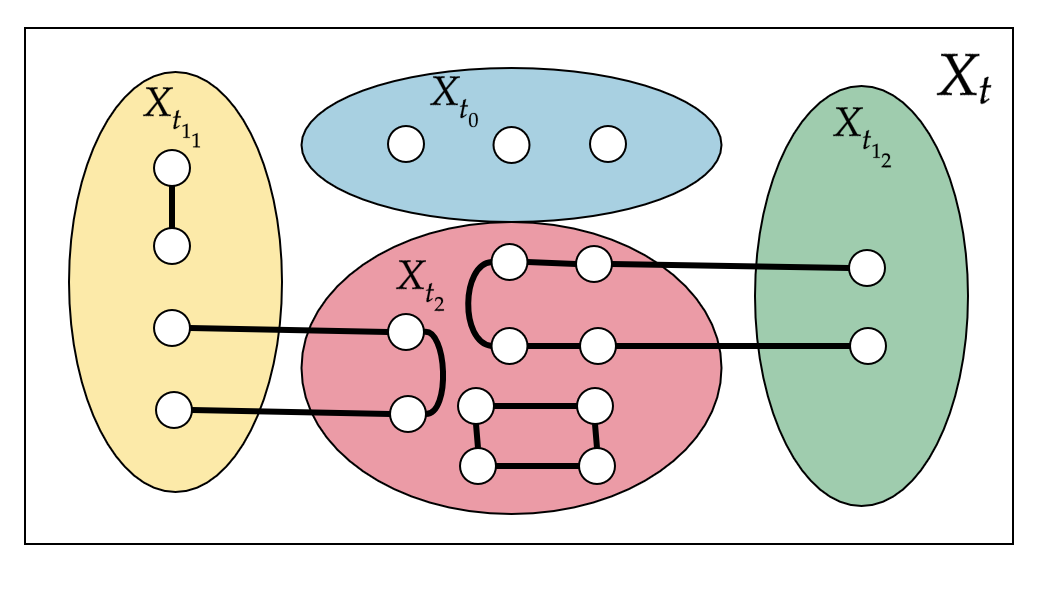
\includegraphics[width=16cm]{cnc_hamiltonian.png}
\caption{$X_t$ ze śladem cyklu Hamiltona.}
\label{cnc_hamiltonian}
\end{figure}
\noindent Dla każdego węzła $t \in V(T)$, funkcji $f: X_t \to \{0,1_1,1_2,2\}$ oraz wagi $w$ rekurencyjnie obliczamy $c(t,f,w)$ będące liczbą par $(H, (V^1, V^2))$, takich że:

\begin{enumerate}[label=(\roman*)]
\item $H$ jest podgrafem $(V_t, E_t)$ oraz $H$ zawiera wszystkie wierzchołki dotychczasowo wprowadzone w bieżącym poddrzewie, tj. $V(H) = V_t$.
\item $(V^1, V^2)$ jest podziałem kompatybilnym z $H$.
\item Funkcja $f$ opisuje przynależność wierzchołków ze zbioru $X_t$ do podzbiorów $X_{t_0}, X_{t_{1_1}}, X_{t_{1_2}}, X_{t_2}$, tj. $X_{t_j} \cap V(H) = f^{-1}(j)$, gdzie $j \in \{0,1_1,1_2,2\}$.
\item Wszystkie wierzchołki ze zbioru $V(H)$ o stopniu 0 należą do $f^{-1}(0)$ (inaczej nieodwołalnie zostawilibyśmy wierzchołek izolowany).
\item Wszystkie wierzchołki ze zbioru $V(H)$ o stopniu 1 należą do $f^{-1}(1_1)$ lub $f^{-1}(1_2)$ (inaczej nieodwołalnie zostawilibyśmy niedomknięty cykl).
\item $\mathbf{w}(H) = w$.
\end{enumerate}

Poniżej przedstawiamy rekurencyjne formuły zależne od typu węzła $t$. Rozwiązanie końcowe zależy od tego, czy istnieje $w$, dla którego wartość $c(r,\emptyset,w) \ mod \ 2$ jest równa $1$. Jeśli tak, to istnieje cykl Hamiltona w grafie $G$. Jeśli nie, to z prawdopodobieństwem co najmniej $\frac{1}{2}$ cykl taki nie istnieje. Wartości funkcji $c$ dla parametrów niezdefiniowanych poniżej wynoszą $0$.
\newline\newline
$t$ jest \texttt{LIŚCIEM}. W tym przypadku algorytm ustawia:
$$c(t,\emptyset,0) = 1.$$
\newline
$t$ jest \texttt{WĘZŁEM WPROWADZAJĄCYM WIERZCHOŁEK} $v$. Wierzchołek $v$ w momencie wprowadzania nie ma incydentnej krawędzi, zatem jeśli $f(v) \neq 0$, to $c(t,f,w) = 0$, wpp.
$$c(t,f,w) = c(t',f_{\big|X_{t'}},w).$$

\begin{table}
\centering
\begin{tabular}{c|c|c|c|c}
 & $0$ & $1_1$ & $1_2$ & $2$ \\
\hline
$0$ & $(1_1,1_1) \vee (1_2,1_2)*$ & $(1_1,2)$ & $(1_2,2)*$ & $\emptyset$ \\
\hline
$1_1$ & $(2,1_1)$ & $(2,2)$ & $\emptyset$ & $\emptyset$ \\
\hline
$1_2$ & $(2,1_2)*$ & $\emptyset$ & $(2,2)$ & $\emptyset$ \\
\hline
$2$ & $\emptyset$ & $\emptyset$ & $\emptyset$ & $\emptyset$ \\
\end{tabular}
\caption{Tabela $tab$ przedstawia przynależność wierzchołków $u$ i $v$ do zbiorów $X_{t_i}$ po dołożeniu krawędzi $uv$, gdzie $u$ odpowiada wierszom, a $v$ kolumnom tabeli. Tabelę należy czytać w następujący sposób: $tab[f'(u)][f'(v)] = (f(u), f(v))$, $f'$ odpowiada funkcji $f$ w węźle $t'$. Gwiazdka* oznacza, że wynik nie jest poprawny dla $v_0$, ponieważ $f(v_0) \neq 1_2$.}
\label{add_edge_table}
\end{table}
\noindent$t$ jest \texttt{WĘZŁEM ZAPOMINAJĄCYM WIERZCHOŁEK} $v$. Wierzchołek może zostać zapomniany wtw. gdy znajduje się w zbiorze $X_{t_2}$, zatem:
$$c(t,f,w) = c(t',f \cup \{(v,2)\},w).$$
\newline
$t$ jest \texttt{WĘZŁEM WPROWADZAJĄCYM KRAWĘDŹ} $uv$. Następujące warunki muszą być spełnione, żeby można było dodać krawędź $uv$ do pokrycia ścieżkowego $G_t$:
\begin{enumerate}[label=(\roman*)]
\item \label{wpr_kr_i}$deg(u) < 2$ oraz $deg(v) < 2$.
\item \label{wpr_kr_ii}$uv$ jest kompatybilna z podziałem $(V^1, V^2)$.
\item \label{wpr_kr_iii}$tab[f'(u)][f'(v)] = (f(u),f(v))$, gdzie $tab$ odnosi się do tabeli \ref{add_edge_table}.  
\end{enumerate}
Zatem mamy:
\[
c(t,f,w) =  
\left \{
  \begin{tabular}{ccc}
  $c(t',f,w) + \sum \limits_{f'} c(t',f',w - w_{uv})$ & jeśli spełnione są warunki \ref{wpr_kr_i}, \ref{wpr_kr_ii}, \ref{wpr_kr_iii},\\
  $c(t',f,w)$ &  wpp.
  \end{tabular}
\right. 
\]

\begin{table}
\centering
\begin{tabular}{c|c|c|c|c}
 & $0$ & $1_1$ & $1_2$ & $2$ \\
\hline
$0$ & $0$ & $1_1$ & $1_2*$ & $2$ \\
\hline
$1_1$ & $1_1$ & $2$ & $\emptyset$ & $\emptyset$ \\
\hline
$1_2$ & $1_2*$ & $\emptyset$ & $2$ & $\emptyset$ \\
\hline
$2$ & $2$ & $\emptyset$ & $\emptyset$ & $\emptyset$ \\
\end{tabular}
\caption{Tabela $tab$ przedstawia przynależność wierzchołka do zbioru $X_{t_i}$ po scaleniu dwóch podgrafów. Tabelę należy interpretować następująco: $tab[f'(v)][f''(v)] = f(v)$, $f'$ i $f''$ odpowiadają funkcji $f$ w węzłach $t'$ i $t''$. Gwiazdka* oznacza, że wynik nie jest poprawny dla $v_0$, ponieważ $f(v_0) \neq 1_2$.}
\label{merge_table}
\end{table}
\noindent$t$ jest \texttt{WĘZŁEM SCALAJĄCYM}. Żeby otrzymać poprawne pokrycie ścieżkowe w wyniku scalenia, muszą zachodzić następujące warunki:
\begin{enumerate}[label=(\roman*)]
\item \label{scal_i}$\forall v \in X_t$: $deg_{t'}(v) + deg_{t''}(v) \leq 2$.
\item Jeśli $f'(v) = 1_i$, to $f''(v) = 1_i$ dla $i \in \{1,2\}$ (kompatybilność sklejanych ścieżek z podziałami).
\item \label{scal_iii}$tab[f'(v)][f''(v)] = f(v)$, gdzie $tab$ odnosi się do tabeli \ref{merge_table}.
\end{enumerate}
Mamy zatem:
$$c(t,f,w) = \sum \limits_{\substack{w' + w'' = w \\ f',f''}} c(t',f',w') \cdot c(t'',f'',w''),$$ gdzie $f'$, $f''$ spełniają warunki \ref{scal_i}-\ref{scal_iii}.

Złożoność powyższego algorytmu wynosi $4^k \cdot n^{\Omicron(1)}$, co poprawia złożoność klasycznego algorytmu działającego w czasie $k^{\Omicron{(k)}} \cdot n^{\Omicron{(1)}}$ dla problemu cyklu Hamiltona.

\newpage
  	\chapter{Porównanie wydajności zaimplementowanych algorytmów}
  	\label{summary}

Wszystkie cztery algorytmy opisane w tej pracy zostały zaimplementowane w języku C++. W tym rozdziale porównamy ich wydajność, opierając się na rezultatach otrzymanych w wyniku przetestowania ich na losowo wygenerowanych drzewach reprezentujących ładne dekompozycje drzewowe grafów wejściowych $G$. Kody źródłowe są umieszczone w repozytorium na githubie \cite{github} i zawierają: 
\begin{itemize}[label=$-$]
\item implementacje klasycznych algorytmów dynamicznych po dekompozycji drzewowej,
\item implementacje algorytmów dynamicznych wykorzystujących technikę Cut \& Count,
\item generator drzew reprezentujących ładne dekompozycje drzewowe grafów wejściowych $G$,
\item eksporter drzew do plików .dot pozwalający wygenerować ich wizualizacje,
\item testy wpisane ręcznie dla małych instancji oraz losowo wygenerowane dla dużych instancji,  
\item generator wykresów porównujących wydajność algorytmów.
\end{itemize}  

Algorytmy pod względem wydajnościowym testowane były wyłącznie na losowo wygenerowanych drzewach, które niekoniecznie stanowią optymalne dekompozycje drzewowe grafów, które reprezentują. Z tego powodu lepszym parametrem opisującym wielkość instancji wejściowych będzie rozmiar drzewa $T$, nie rozmiar grafu $G$.

Dla problemu Drzewa Steinera algorytmy klasyczny i probabilistyczny zostały wykonane na instancjach drzew o rozmiarach: 51, 91, 96 i odpowiednio o  następujących szerokościach drzewowych: 4, 5, 6. Każdy wierzchołek z jednakowym prawdopodobieństwem równym 0.5 był wybierany do zbioru terminali $K \subset V(G)$. Krawędzie były dobierane do grafu $G$ na samym końcu, kiedy wszystkie inne węzły $T$ były już wygenerowane. Poniżej węzła $t$ zapominającego $v$, dodawane były prawie wszystkie krawędzie $uv$, takie że $u \in X_t$. Wykres \ref{steiner_test_time} przedstawia uzyskane wyniki. Łatwo zaobserwować znaczną przewagę algorytmu probabilistycznego z użyciem techniki Cut \& Count nad klasycznym algorytmem dynamicznym po dekompozycji drzewowej. Dla szerokości drzewowej równej 7 algorytm probabilistyczny zadziałał w granicach 5 sekund, podczas gdy algorytm klasyczny nie skończył działania w rozsądnym przedziale czasowym. 

\begin{figure}
\centering
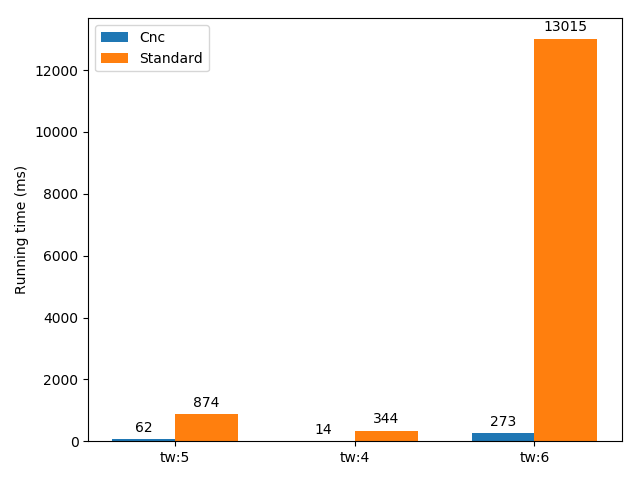
\includegraphics[width=14cm]{steiner_test_time.png}
\caption{Porównanie czasu działania algorytmów dla problemu Drzewa Steinera.}
\label{steiner_test_time}
\end{figure}

Dla problemu Cyklu Hamiltona testy zostały przeprowadzone na drzewach o rozmiarach: 51, 91, 96 i odpowiednio następujących szerokościach drzewowych: 4, 5, 6. Schemat generowania krawędzi grafu $G$ był jednakowy jak poprzednio. Analiza porównawcza algorytmu klasycznego i algorytmu probabilistycznego prowadzi do innych wniosków niż w przypadku problemu Drzewa Steinera. Okazuje się, że czasy działania algorytmów na instancjach o mniejszych szerokościach drzewowych są zbliżone, natomiast dla instancji o szerokości drzewowej równej 6 algorytm probabilistyczny działa dwa razy wolniej. Prawdopodobnie wynika to z tego, że ślady cyklu Hamiltona w poddrzewach są większe niż ślady drzewa Steinera dla instancji o podobnych rozmiarach. Jest to następstwem tego, że w problemie Cyklu Hamiltona możemy na każdy wierzchołek patrzeć jak na terminal, który docelowo musi mieć dwie krawędzie do niego incydentne. Większa liczba krawędzi generuje więcej śladów o różnych wagach, których liczba znacząco wpływa na wydajność działania algorytmów bazujących na technice Cut \& Count.

Warto również nadmienić, że w kontekście implementacji algorytmy z użyciem techniki Cut \& Count są znacznie prostsze i krótsze od algorytmów klasycznych, co jest ich niewątpliwą zaletą.

\begin{figure}
\centering
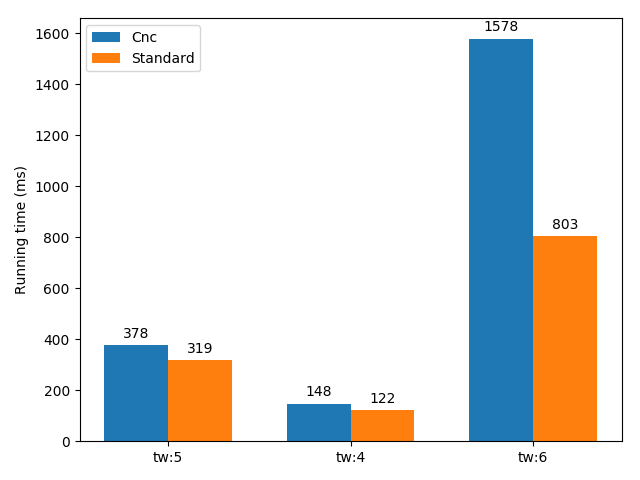
\includegraphics[width=14cm]{hamiltonian_test_time.png}
\caption{Porównanie czasu działania algorytmów dla problemu Cyklu Hamiltona.}
\label{hamiltonian_test_time}
\end{figure}


\newpage
	\begin{thebibliography}{9}
		\bibitem{parametrized_algorithms}
			M. Cygan, F. V. Fomin, Ł. Kowalik, D. Lokshtanov, D. Marx, M. Pilipczuk, M. Pilipczuk, S. Saurabh
 			\textit{Parameterized Algorithms}.
 			
 		\bibitem{solving_connectivity_problems}
 			Cygan, M., Nederlof, J., Pilipczuk, M., Pilipczuk, M., van Rooij, J.M.M., Wojtaszczyk,
J.O.
			\textit{Solving connectivity problems parameterized by treewidth in single
exponential time}
			Proceedings of the 52nd Annual Symposium on Foundations of Computer Science (FOCS), pp. 150-159. IEEE (2011)
 					
		\bibitem{bodlaender}  
			H. L. Bodlaender. 
			\textit{A linear-time algorithm for finding tree-decompositions of small treewidth}. 
			SIAM J. Comput. 25:6 (1996) 1305-1317		
		
		\bibitem{kloks} 
			T. Kloks. 
			\textit{Treewidth. Computations and approximations}. 
			Lecture Notes in Computer Science, 842, 1994.
 			
		\bibitem{github} 
			P. Kyzioł. Cut \& Count - Code repository, 2019
			\\\texttt{https://github.com/polapl/Cut-and-Count}
	\end{thebibliography} 



\end{document}
